Nous avons commencé ce projet en ne travaillant que sur des images en niveaux de gris. Cependant, les résultats présentés ci-dessus sont en couleur. Afin de résoudre le problème sur ce type d'image, nous avons décidé d'utiliser l'espace RGB (Red Green Blue).
\subsection{De l'image en niveaux de gris...}
Une image  en niveaux de gris, peut être considérée comme une matrice dont chaque pixel possède une valeur comprise entre 0 (noir) et 255 (blanc), les valeurs intermédiaires représentant un niveau de gris. Une image couleur se distingue d'une image en "noir et blanc" par le nombre de "canaux" qu'elle possède. Dans le cas d'image au format RGB, l'image possède 3 canaux.\\ Les canaux Rouge, Vert et Bleu, respectivement.\\
L'image obtenue, affichée sur l'écran, est donc une superposition de ses canaux.
 Un canal est la matrice associée à une couleur (Rouge, Vert ou Bleu), les valeurs de cette matrice étant comprises entre 0 et 255, il permet de caractériser la composante (R V ou B) de l'image. \\ 
 \begin{figure}[H]
 \centering
 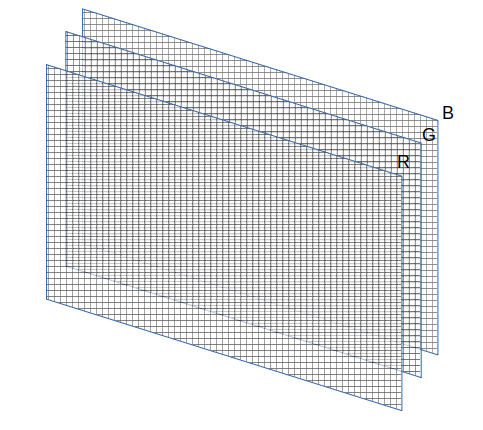
\includegraphics[scale=0.2]{Images/rgb.png}
 \caption{Superposition des matrices}
 \end{figure}
Afin de résoudre le problème sur des images en couleur, nous avons donc appliqué les mêmes algorithmes que ceux utilisés pour une image en niveaux de gris sur chacune des matrices R G et B.
L'algorithme est appliqué sur chaque canal de l'image.\\
 \begin{figure}[H]
 \centering
 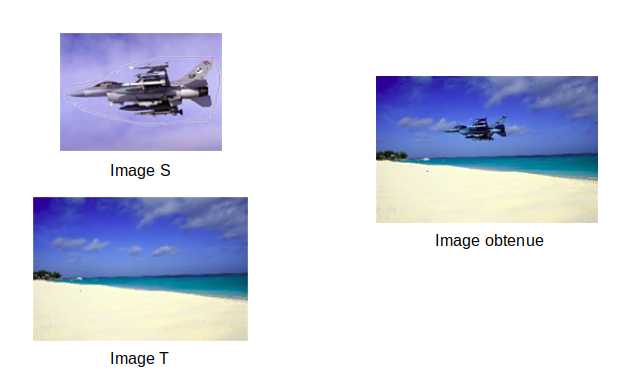
\includegraphics[scale=0.5]{Images/couleur.png}
 \caption{Image obtenue avec l'algorithme des différences finies}
 \end{figure}
Cependant, en observant les résultats obtenus plus haut, il est clair que la couleur de l'objet collé sur l'image finale est souvent "dénaturée", trop saturée.\\
En observant l'exemple ci-dessus, l'avion présent dans l'image S, avec une couleur initiale que l'on pourrait considérée comme "grise" se retrouve dans l'image finale avec une couleur "bleue" s'accordant avec le ciel. L'image obtenue dénature alors la couleur de l'objet à coller.  L'espace RGB, qui utilise les systèmes de synthèse additive, ne semble donc pas un espace à utiliser pour faire ce genre de  traitement d'images. \\
Afin de résoudre ce problème nous aurions pu utiliser un autre espace de couleurs, l'espace HSL (Hue Saturation Lightness ou Teinte Saturation luminosité en français). Dans ce nouvel espace il est possible d'influer sur : 
\begin{itemize}
\item La saturation de l'image: l'intensité des couleurs qu'elle possède.
\item  La teinte  :  la couleur de l'image.
\item La luminosité : la lumière présente dans l'image
\end{itemize} 
Cet espace est beaucoup plus intéressant que celui précédemment utilisé. En effet, il est possible grâce à lui, d'influer sur plus de paramètres que sur l'espace RGB. Nous pouvons donc la saturation de l'image objet ainsi que sa luminosité, sans dénaturer la couleur de celui-ci, comme ce fut le cas dans de nombreux de nos essais avec l'espace RGB. \cite{Couleur}